\documentclass[a4paper, 12pt]{article}

% packages
\usepackage{amssymb}
\usepackage[fleqn]{mathtools}
\usepackage{tikz}
\usepackage{enumerate}
\usepackage{bussproofs}
\usepackage{xcolor}
\usepackage[margin=1.3cm]{geometry}
\usepackage{logicproof}
\usepackage{diagbox}
\usepackage{listings}
\usepackage{graphicx}
\usepackage{lstautogobble}
\usepackage{hyperref}
\usepackage{multirow}
\usepackage{tipa}
\usepackage{pgfplots}

% tikz libraries
\usetikzlibrary{
    decorations.pathreplacing,
    arrows,
    shapes.gates.logic.US,
    circuits.logic.US,
    calc,
    automata,
    positioning,
    intersections
}

\pgfplotsset{compat=1.16}

\pgfmathdeclarefunction{gauss}{2}{%
  \pgfmathparse{1/(#2*sqrt(2*pi))*exp(-((x-#1)^2)/(2*#2^2))}%
}

\allowdisplaybreaks % allow environments to break
\setlength\parindent{0pt} % no indent

% shorthand for verbatim
% this clashes with logicproof, so maybe fix this at some point?
\catcode`~=\active
\def~#1~{\texttt{#1}}

% code listing
\lstdefinestyle{main}{
    numberstyle=\tiny,
    breaklines=true,
    showspaces=false,
    showstringspaces=false,
    tabsize=2,
    numbers=left,
    basicstyle=\ttfamily,
    columns=fixed,
    fontadjust=true,
    basewidth=0.5em,
    autogobble,
    xleftmargin=3.0ex,
    mathescape=true
}
\newcommand{\dollar}{\mbox{\textdollar}} %
\lstset{style=main}

% augmented matrix
\makeatletter
\renewcommand*\env@matrix[1][*\c@MaxMatrixCols c]{%
\hskip -\arraycolsep
\let\@ifnextchar\new@ifnextchar
\array{#1}}
\makeatother

% ceiling / floor
\DeclarePairedDelimiter{\ceil}{\lceil}{\rceil}
\DeclarePairedDelimiter{\floor}{\lfloor}{\rfloor}

% custom commands
\newcommand{\indefint}[2]{\int #1 \, \mathrm{d}#2}
\newcommand{\defint}[4]{\int_{#1}^{#2} #3 \, \mathrm{d}#4}
\newcommand{\pdif}[2]{\frac{\partial #1}{\partial #2}}
\newcommand{\dif}[2]{\frac{\mathrm{d}#1}{\mathrm{d}#2}}
\newcommand{\limit}[2]{\raisebox{0.5ex}{\scalebox{0.8}{$\displaystyle{\lim_{#1 \to #2}}$}}}
\newcommand{\limitsup}[2]{\raisebox{0.5ex}{\scalebox{0.8}{$\displaystyle{\limsup_{#1 \to #2}}$}}}
\newcommand{\summation}[2]{\sum\limits_{#1}^{#2}}
\newcommand{\product}[2]{\prod\limits_{#1}^{#2}}
\newcommand{\intbracket}[3]{\left[#3\right]_{#1}^{#2}}
\newcommand{\laplace}{\mathcal{L}}
\newcommand{\fourier}{\mathcal{F}}
\newcommand{\mat}[1]{\boldsymbol{#1}}
\renewcommand{\vec}[1]{\boldsymbol{#1}}
\newcommand{\rowt}[1]{\begin{bmatrix}
    #1
\end{bmatrix}^\top}
\DeclareMathOperator*{\argmax}{argmax}
\DeclareMathOperator*{\argmin}{argmin}

\newcommand{\lto}[0]{\leadsto\ }

\newcommand{\ulsmash}[1]{\underline{\smash{#1}}}

\newcommand{\powerset}[0]{\wp}
\renewcommand{\emptyset}[0]{\varnothing}

\makeatletter
\newsavebox{\@brx}
\newcommand{\llangle}[1][]{\savebox{\@brx}{\(\m@th{#1\langle}\)}%
  \mathopen{\copy\@brx\kern-0.5\wd\@brx\usebox{\@brx}}}
\newcommand{\rrangle}[1][]{\savebox{\@brx}{\(\m@th{#1\rangle}\)}%
  \mathclose{\copy\@brx\kern-0.5\wd\@brx\usebox{\@brx}}}
\makeatother
\newcommand{\lla}{\llangle}
\newcommand{\rra}{\rrangle}
\newcommand{\la}{\langle}
\newcommand{\ra}{\rangle}
\newcommand{\crnr}[1]{\text{\textopencorner} #1 \text{\textcorner}}
\newcommand{\bnfsep}[0]{\ |\ }
\newcommand{\concsep}[0]{\ ||\ }

\newcommand{\axiom}[1]{\AxiomC{#1}}
\newcommand{\unary}[1]{\UnaryInfC{#1}}
\newcommand{\binary}[1]{\BinaryInfC{#1}}
\newcommand{\trinary}[1]{\TrinaryInfC{#1}}
\newcommand{\quaternary}[1]{\QuaternaryInfC{#1}}
\newcommand{\quinary}[1]{\QuinaryInfC{#1}}
\newcommand{\dproof}[0]{\DisplayProof}

\newcommand{\ttbs}{\char`\\}
\newcommand{\lrbt}[0]{\ \bullet\ }

% colours
\newcommand{\violet}[1]{\textcolor{violet}{#1}}
\newcommand{\blue}[1]{\textcolor{blue}{#1}}
\newcommand{\red}[1]{\textcolor{red}{#1}}
\newcommand{\teal}[1]{\textcolor{teal}{#1}}

% reasoning proofs
\usepackage{ltablex}
\usepackage{environ}
\keepXColumns
\NewEnviron{reasoning}{
    \begin{tabularx}{\textwidth}{rlX}
        \BODY
    \end{tabularx}
}
\newcommand{\proofline}[3]{$(#1)$ & $#2$ & \hfill #3 \smallskip \\}
\newcommand{\proofarbitrary}[1]{& take arbitrary $#1$ \smallskip \\}
\newcommand{\prooftext}[1]{\multicolumn{3}{l}{#1} \smallskip \\}
\newcommand{\proofmath}[3]{$#1$ & = $#2$ & \hfill #3 \smallskip \\}
\newcommand{\prooftherefore}[1]{& $\therefore #1$ \smallskip \\}
\newcommand{\proofbc}[0]{\prooftext{\textbf{Base Case}}}
\newcommand{\proofis}[0]{\prooftext{\textbf{Inductive Step}}}

% ER diagrams
\newcommand{\nattribute}[4]{
    \node[draw, state, inner sep=0cm, minimum size=0.2cm, label=#3:{#4}] (#1) at (#2) {};
}
\newcommand{\mattribute}[4]{
    \node[draw, state, accepting, inner sep=0cm, minimum size=0.2cm, label=#3:{#4}] (#1) at (#2) {};
}
\newcommand{\dattribute}[4]{
    \node[draw, state, dashed, inner sep=0cm, minimum size=0.2cm, label=#3:{#4}] (#1) at (#2) {};
}
\newcommand{\entity}[3]{
    \node[] (#1-c) at (#2) {#3};
    \node[inner sep=0cm] (#1-l) at ($(#1-c) + (-1, 0)$) {};
    \node[inner sep=0cm] (#1-r) at ($(#1-c) + (1, 0)$) {};
    \node[inner sep=0cm] (#1-u) at ($(#1-c) + (0, 0.5)$) {};
    \node[inner sep=0cm] (#1-d) at ($(#1-c) + (0, -0.5)$) {};
    \draw
    ($(#1-c) + (-1, 0.5)$) -- ($(#1-c) + (1, 0.5)$) -- ($(#1-c) + (1, -0.5)$) -- ($(#1-c) + (-1, -0.5)$) -- cycle;
}
\newcommand{\relationship}[3]{
    \node[] (#1-c) at (#2) {#3};
    \node[inner sep=0cm] (#1-l) at ($(#1-c) + (-1, 0)$) {};
    \node[inner sep=0cm] (#1-r) at ($(#1-c) + (1, 0)$) {};
    \node[inner sep=0cm] (#1-u) at ($(#1-c) + (0, 1)$) {};
    \node[inner sep=0cm] (#1-d) at ($(#1-c) + (0, -1)$) {};
    \draw
    ($(#1-c) + (-1, 0)$) -- ($(#1-c) + (0, 1)$) -- ($(#1-c) + (1, 0)$) -- ($(#1-c) + (0, -1)$) -- cycle;
}

\newcommand{\avltri}[4]{
    \draw ($(#1)$) -- ($(#1) + #4*(0.5, -1)$) -- ($(#1) + #4*(-0.5, -1)$) -- cycle;
    \node at ($(#1) + #4*(0, -1) + (0, 0.5)$) {#3};
    \node at ($(#1) + #4*(0, -1) + (0, -0.5)$) {#2};
}

% actual document
\begin{document}
    \section*{CO202 - Algorithms II}
        \subsection*{8th October 2019}
            \subsubsection*{Introduction}
                Note that this course is taught in Haskell, and in the style of Dijkstra (structure of algorithms), instead of Knuth (analysis and complexity).
            \subsubsection*{List Insertion}
                An algorithm to insert elements in a sorted list;
                \begin{lstlisting}
                    insert :: Int -> [Int] -> [Int]
                    insert x [] = [x]
                    insert x (y:ys)
                      | x <= y    = x:y:ys
                      | otherwise = y:insert x ys
                \end{lstlisting}
                In Haskell, we do this by case analysis, first looking at the base case (line 2) - where the list is empty.
                The second case (line 3) considers the non-empty list.
                The evaluation is as follows, for a simple example;
                \begin{align*}
                    & ~insert 4 [1,3,6,7,9]~ \\
                    \lto & ~1:insert 4 [3,6,7,9]~ & \text{definition of ~insert~} \\
                    \lto & ~1:3:insert 4 [6,7,9]~ & \text{definition of ~insert~} \\
                    \lto & ~1:3:4:6:[7,9]~ & \text{definition of ~insert~}
                \end{align*}
                To give a cost, we will measure the number of steps, which approximates time - the number of steps is essentially each transition from the LHS of ~=~ to the RHS.
                The measure of input will be $n = ~length xs~$.
                We write a recurrence relationship that ties together$n$ with the algorithm;
                \begin{align*}
                    T(0) & = 1 & \text{1 transition} \\
                    T(n) & = 1 + T(n - 1) & \text{looking at worst case, line 5}
                \end{align*}
                The structure of the complexity should follow the structure of the algorithm itself.
                However, we are interested in a closed form for $T(n)$, where we can directly obtain the value without evaluating recursively.
                The easiest way to do this is to unroll the definition, and look for patterns;
                \begin{align*}
                    T(n) & = 1 + T(n - 1) \\
                    & = 1 + (1 + T(n - 2)) \\
                    & = 1 + (1 + \dots + T(n - n)) \\
                    & = 1 + n
                \end{align*}
            \subsubsection*{Insertion Sort}
                The previous algorithm can be used as the basis for insertion sort.
                For each element in the unsorted list, we insert it into the sorted list (which is initially empty).
                \begin{lstlisting}
                    isort :: [Int] -> [Int]
                    isort [] = []
                    isort (x:xs) = insert x (isort xs)
                \end{lstlisting}
                We assume that ~insert~, and ~isort~ both give us a sorted list, assuming the input lists were also sorted.
                An example of this on a small list is as follows;
                \begin{align*}
                    & ~isort [3,1,2]~ \\
                    \lto & ~insert 3 (isort [1,2])~ & \text{definition of ~isort~} \\
                    \lto & ~insert 3 (insert 1 (isort [2]))~ & \text{definition of ~isort~} \\
                    \lto & ~insert 3 (insert 1 (insert 2 (isort [])))~ & \text{definition of ~isort~} \\
                    \lto & ~insert 3 (insert 1 (insert 2 []))~ & \text{definition of ~isort~} \\
                    \lto & ~insert 3 (insert 1 [2])~ & \text{definition of ~insert~} \\
                    \lto & ~insert 3 (1:2:[])~ & \text{definition of ~insert~} \\
                    \lto & ~1:insert 3 (2:[])~ & \text{definition of ~insert~} \\
                    \lto & ~1:2:(insert 3 [])~ & \text{definition of ~insert~} \\
                    \lto & ~1:2:[3]~ & \text{definition of ~insert~}
                \end{align*}
                This cost 9 steps to evaluate.
                The recurrence relation generalises this (similarly $n = ~length xs~$);
                \begin{align*}
                    T_~isort~(0) & = 1 \\
                    T_~isort~(n) & = 1 + T_~insert~(n - 1) + T_~isort~(n - 1)
                    \intertext{However, we want to find this in closed form;}
                    T_~isort~(n) & = 1 + n + T_~isort~(n - 1) \\
                    & = 1 + n + (1 + n - 1 + T_~isort~(n - 2)) \\
                    & = \dots \\
                    & = \frac{n (n + 1)}{2} + 1 + n
                \end{align*}
                A more thorough analysis will teach us about;
                \begin{itemize}
                    \itemsep0em
                    \item evaluation strategies and cost
                    \item counting carefully and crudely
                    \item abstract interfaces
                    \item data structures
                \end{itemize}
        \subsection*{11th October 2019}
            \subsubsection*{Laziness}
                In the last lecture, we saw ~isort~ sorts in approximately $n^2$ steps.
                \begin{lstlisting}
                    minimum :: [Int] -> Int
                    minimum = head . isort
                \end{lstlisting}
                The evaluation of ~minimum~ takes $n$ steps, when given a sorted list;
                \begin{align*}
                    & ~minimum [1,2,3]~ \\
                    \lto & ~head (sort [1,2,3])~ \\
                    \lto & \dots \\
                    \lto & ~head (insert 1 (insert 2 (insert 3 [])))~ \\
                    \lto & ~head (insert 1 (insert 2 [3]))~ \\
                    \lto & ~head (insert 1 (2:[3]))~ \\
                    \lto & ~head 1:2:[3]~ \\
                    \lto & ~1~
                \end{align*}
                The worst case is a reversed list, as follows;
                \begin{align*}
                    & ~minimum [3,2,1]~ \\
                    \lto & ... \\
                    \lto & ~head (insert 3 (insert 2 (insert 1 [])))~ \\
                    \lto & ~head (insert 3 (insert 2 [1]))~ \\
                    \lto & ~head (insert 3 (1:insert 2 []))~ \\
                    \lto & ~head (1:insert 3 (insert 2 []))~
                \end{align*}
                The important part is to note that the minimum value, ~1~, is floated to the left, for a total of $n$ steps.
                Therefore, this still takes linear time.
                This evaluation relies on laziness, hence we can build the large computation on the RHS of the ~:~.
            \subsubsection*{Normal Forms}
                There are three normal forms that values can take;
                \begin{itemize}
                    \itemsep0em
                    \item \textbf{normal form (NF)}
                        \medskip

                        This is fully evaluated, and there is no more work to be done - an expression is in NF if it is;
                        \begin{itemize}
                            \itemsep0em
                            \item a constructor applied to arguments in NF
                            \item a $\lambda$-abstraction (function) whose body is in NF
                        \end{itemize}
                    \item \textbf{head normal form (HNF)}
                        \medskip

                        An expression is in HNF if it is;
                        \begin{itemize}
                            \itemsep0em
                            \item a constructor applied to arguments in any form
                            \item a $\lambda$-abstraction (function) whose body is in HNF
                        \end{itemize}
                    \item \textbf{weak head normal form (WHNF)}
                        \medskip

                        An expression is in WHNF if it is;
                        \begin{itemize}
                            \itemsep0em
                            \item a constructor applied to arguments in any form
                            \item a $\lambda$-abstraction (function) whose body is in any form
                        \end{itemize}
                \end{itemize}
                Looking at the last line in the previous evaluation, we have two constructors; cons (~:~) and the empty list (~[]~).
                The LHS of ~:~ is in normal form, but the RHS isn't, and therefore it cannot be in normal form.
            \subsubsection*{Evaluation Order}
                There are two main evaluation strategies;
                \begin{itemize}
                    \itemsep0em
                    \item \textbf{applicative order} (eager / strict evaluation) \hfill goes to normal form
                        \medskip

                        Evaluates as much as possible, until it ends up in normal form.
                        It evaluates the left-most, inner-most expression first.
                        For example, in the final step ~head (1:insert 3 (insert 2 []))~, it would first evaluate ~2~, then ~[]~, and then ~insert 2 []~, and so on.
                    \item \textbf{normal order} (lazy evaluation) \hfill goes to weak head normal form
                        \medskip

                        This evaluates the left-most, outer-most expression first.
                \end{itemize}
            \subsubsection*{Counting Carefully}
                Here we are concerned at counting the steps mechanically in strict evaluation.
                This is done for a simplified language, containing constants, variables, functions, conditionals, and pattern matching.
                We will write $e^T$ to denote the number of steps it takes to reduce $e$.
                Additionally, if $f$ is a primitive function, then $f^T\ e_1\ \dots\ e_n = 0$, otherwise $f\ e_1\ \dots\ e_n = e$, and $f^T\ e_1\ \dots\ e_n = 1 + e^T$.
                \begin{align*}
                    k^T & = 0 & \text{constants} \\
                    x^T & = 0 & \text{evaluated variables} \\
                    (f\ e_1\ \dots\ e_n)^T & = (f^T\ e_1\ \dots\ e_n) + e_1^T + \dots + e_n^T & \text{function with arguments} \\
                    (~if ~ p ~ then ~ e_1 ~ else ~ e_2)^T & = p^T + (~if ~ p ~ then ~ e_1^T ~ else ~ e_2^T) & \text{conditional} \\
                   \left(~case ~ e ~ of ~ \begin{cases}
                       p_1 & \to e_1 \\
                       & \vdots \\
                       p_n & \to e_n
                   \end{cases} \right)^T & = e^T + \left(~case ~ e ~ of ~ \begin{cases}
                        p_1 & \to e_1^T \\
                        & \vdots \\
                        p_n & \to e_n^T
                    \end{cases}\right) & \text{pattern matching}
                \end{align*}
                This is very involved for tiny examples, and becomes much more complex for lazy evaluation.
            \subsubsection*{Counting Crudely}
                We mainly use asymptotic notation to achieve this.
                Certain functions dominate others when given enough time - as the input increases.
                \medskip

                L-functions are the smallest class of one-valued functions on real variables $n \in \mathbb{R}$, containing constants, the variable $n$, and are closed under arithmetic, exponentiation, and logarithms.
                They tend to be monotonic after a given time, and tend to a value.
                \medskip

                Consider $f(n) = 2n$, and $g(n) = \frac{n^2}{4}$ - at $n = 1$, $f(1) > g(1)$, however at some point on the number line, $g$ begins to dominate.
                Comparing functions can be achieved by studying their ratios (with well-behaved functions, like L-functions, the ratio will tend to 0, infinity, or a constant);
                $$\limit{n}{\infty} \frac{f(n)}{g(n)}$$
                Any L-function is ultimately continuous of constant sign, monotonic, and approaches 0, $\infty$, or some definite limit as $n \to \infty$.
                Furthermore, $\frac{f}{g}$ is an L-function if both $f$ and $g$ are.
                We can now introduce notation compare function;
                \begin{align*}
                    f \prec g & \triangleq \limit{n}{\infty} \frac{f(n)}{g(n)} = 0 & \text{also written as } f \in o(g(n)) \\
                    f \preceq g & \triangleq \limitsup{n}{\infty} \frac{f(n)}{g(n)} < \infty & \text{also written as } f \in O(g(n)) \\
                    f \asymp g & \triangleq f \in (O(g(n)) \cap \Omega(g(n))) & \text{also written as } f \in \Theta(g(n)) \\
                    f \succeq g & \triangleq \limitsup{n}{\infty} \left|\frac{f(n)}{g(n)}\right| > 0 & \text{also written as } f \in \Omega(g(n)) \\
                    f \succ g & \triangleq \limit{n}{\infty} \left|\frac{f(n)}{g(n)}\right| = \infty & \text{also written as } f \in \omega(g(n))
                \end{align*}
                Visually, we can represent this in the following three graphs.
                Note that $\delta, \delta_1, \delta_2$ are just constant multipliers.
                The first plot shows that as $n$ gets larger $f(n)$ will exist within the shaded region bounded above by $\delta g(n)$, and similarly (on the other extreme) the third plot shows that as $n$ gets larger, $f(n)$ will exist within the region bounded below by $\delta g(n)$.
                If $f$ is constrained (as time progresses) within the region bounded by $\delta_1 g(n)$ and $\delta_2 g(n)$, then we have the second plot.
                \begin{center}
                    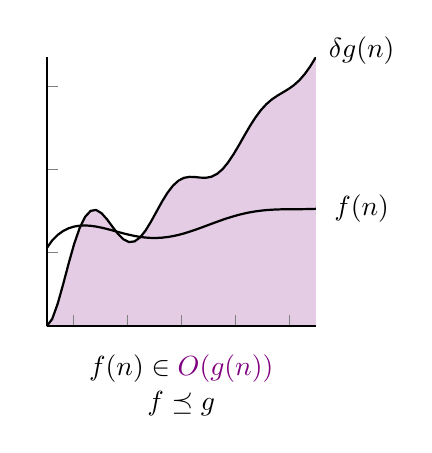
\begin{tikzpicture}
                        \begin{axis}[
                            axis on top=true,
                            axis line style=thick,
                            no markers, domain=1:11, samples=50,
                            axis lines*=left, xlabel=\shortstack{$f(n) \in \violet{O(g(n))}$\\$f \preceq g$}, ylabel=,
                            height=5cm, width=5cm,
                            enlargelimits=false,
                            xticklabels={,,},
                            yticklabels={,,}
                        ]
                            \addplot[fill=violet!20, draw=none] {10 + 0.2*\x^2 + 10*sin(deg(2*(x - 2)))/x} \closedcycle;
                            \addplot[thick] {10 + 0.2*\x^2 + 10*sin(deg(2*(x - 2)))/x};
                            \addplot[thick] {10 + 0.5*\x + 5*sin(deg(x - 1))/x};
                        \end{axis}
                        \node at (4, 3.5) {$\delta g(n)$};
                        \node at (4, 1.5) {$f(n)$};
                    \end{tikzpicture}
                    \hfill
                    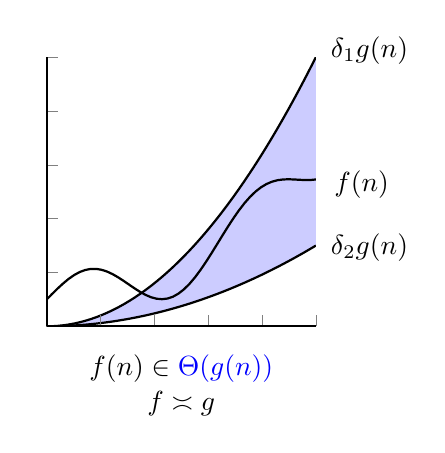
\begin{tikzpicture}
                        \begin{axis}[
                            axis on top=true,
                            axis line style=thick,
                            no markers, domain=0:10, samples=50,
                            axis lines*=left, xlabel=\shortstack{$f(n) \in \blue{\Theta(g(n))}$\\$f \asymp g$}, ylabel=,
                            height=5cm, width=5cm,
                            enlargelimits=false,
                            xticklabels={,,},
                            yticklabels={,,}
                        ]
                            \addplot[fill=blue!20, draw=none] {0.1*\x^2} \closedcycle;
                            \addplot[fill=white, draw=none] {0.03*\x^2} \closedcycle;
                            \addplot[thick] {0.1*\x^2};
                            \addplot[thick] {0.03*\x^2};
                            \addplot[thick] {1 + 0.05*\x^2 + sin(deg(x))};
                        \end{axis}
                        \node at (4.1, 3.5) {$\delta_1 g(n)$};
                        \node at (4.1, 1) {$\delta_2 g(n)$};
                        \node at (4, 1.8) {$f(n)$};
                    \end{tikzpicture}
                    \hfill
                    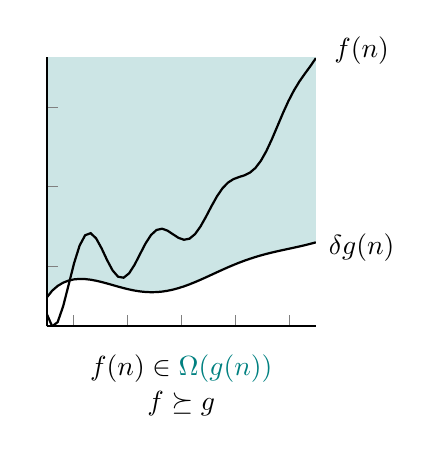
\begin{tikzpicture}
                        \begin{axis}[
                            axis on top=true,
                            axis line style=thick,
                            no markers, domain=1:11, samples=50,
                            axis lines*=left, xlabel=\shortstack{$f(n) \in \teal{\Omega(g(n))}$\\$f \succeq g$}, ylabel=,
                            height=5cm, width=5cm,
                            enlargelimits=false,
                            xticklabels={,,},
                            yticklabels={,,}
                        ]
                            \addplot[fill=teal!20, draw=none] {36.3} \closedcycle;
                            \addplot[fill=white, draw=none] {6 + 0.06*\x^2 + 5*sin(deg(x - 1))/x} \closedcycle;
                            \addplot[thick] {10 + 0.02*\x^3 + 10*sin(deg(2.5*(x - 2)))/x};
                            \addplot[thick] {6 + 0.06*\x^2 + 5*sin(deg(x - 1))/x};
                        \end{axis}
                        \node at (4, 3.5) {$f(n)$};
                        \node at (4, 1) {$\delta g(n)$};
                    \end{tikzpicture}
                \end{center}
                If $f$ and $g$ are L-functions, then either;
                \begin{center}
                    $f \in o(g)$, $f \in \Theta(g)$, or $f \in \Omega(g)$
                \end{center}
                Another method of visualising this is as a Venn diagram, with the upper circle being $O(g(n))$, and the lower circle being $\Omega(g(n))$;
                \begin{center}
                    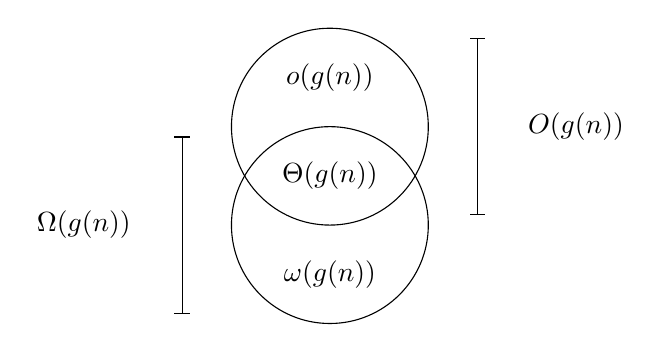
\begin{tikzpicture}[x=1.25cm, y=1.25cm]
                        \draw (0, 0) circle (1);
                        \draw (0, -1) circle (1);
                        \node at (0, 0.5) {$o(g(n))$};
                        \node at (0, -0.5) {$\Theta(g(n))$};
                        \node at (0, -1.5) {$\omega(g(n))$};
                        \node at (2.5, 0) {$O(g(n))$};
                        \node at (-2.5, -1) {$\Omega(g(n))$};
                        \draw
                        (1.5, 0.9) edge[|-|] (1.5, -0.9)
                        (-1.5, -0.1) edge[|-|] (-1.5, -1.9);
                    \end{tikzpicture}
                \end{center}
                Finally, this can also be defined by the following;
                \begin{align*}
                    o(g(n)) & = \{ f \bnfsep \forall \delta > 0.\ \exists n_0 > 0.\ \forall n > n_0.\ |f(n)| < \delta g(n) \} \\
                    O(g(n)) & = \{ f \bnfsep \violet{\exists \delta > 0.\ \exists n_0 > 0.\ \forall n > n_0.\ |f(n)| \leq \delta g(n)} \} \\
                    \Theta(g(n)) & = \left\{f\ \left|\ \begin{matrix}
                        (\violet{\exists \delta > 0.\ \exists n_0 > 0.\ \forall n > n_0.\ |f(n)| \leq \delta g(n)}) \\
                        \land \\
                        (\teal{\exists \delta > 0.\ \forall n_0 > 0.\ \exists n > n_0.\ f(n) \geq \delta g(n)})
                    \end{matrix}\right.\right\} \\
                    & = O(g(n)) \cap \Omega(g(n)) \\
                    \Omega(g(n)) & = \{f \bnfsep \teal{\exists \delta > 0.\ \forall n_0 > 0.\ \exists n > n_0.\ f(n) \geq \delta g(n)}\} \\
                    \omega(g(n)) & = \{ f \bnfsep \forall \delta > 0.\ \forall n_0 > 0.\ \exists n > n_0.\ f(n) > \delta g(n) \}
                \end{align*}
        \subsection*{15th October 2019}
            \subsubsection*{Basic Lists}
                In Haskell, lists are given by \textbf{two} constructors;
                \begin{lstlisting}
                    data [a] = [] | (:) a [a]
                \end{lstlisting}
                This creates two values, called constructors (RHS of data declaration, hence we can pattern match on these unlike other functions);
                \begin{lstlisting}
                    [] :: [a]
                    (:) :: a -> [a] -> [a]
                \end{lstlisting}
                In Haskell, data structures are persistent by default.
                \begin{center}
                    ~[x1,x2,x3] = x1:x2:x3:[]~
                \end{center}
                Visually, we can look at this as "cells" with their constructors and arguments;
                \begin{center}
                    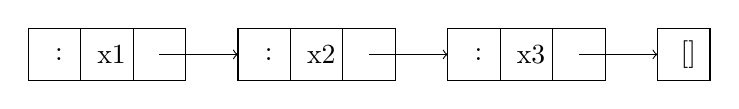
\begin{tikzpicture}[x=0.666cm, y=0.666cm]
                        \begin{scope}[shift={(0, 0)}]
                            \node at (0.5, -0.5) {~:~};
                            \node at (1.5, -0.5) {~x1~};
                            \draw
                            (0, 0) -- (3, 0) -- (3, -1) -- (0, -1) --cycle
                            (1, 0) -- (1, -1)
                            (2, 0) -- (2, -1)
                            (2.5, -0.5) edge[->] (4, -0.5);
                        \end{scope}
                        \begin{scope}[shift={(4, 0)}]
                            \node at (0.5, -0.5) {~:~};
                            \node at (1.5, -0.5) {~x2~};
                            \draw
                            (0, 0) -- (3, 0) -- (3, -1) -- (0, -1) --cycle
                            (1, 0) -- (1, -1)
                            (2, 0) -- (2, -1)
                            (2.5, -0.5) edge[->] (4, -0.5);
                        \end{scope}
                        \begin{scope}[shift={(8, 0)}]
                            \node at (0.5, -0.5) {~:~};
                            \node at (1.5, -0.5) {~x3~};
                            \draw
                            (0, 0) -- (3, 0) -- (3, -1) -- (0, -1) --cycle
                            (1, 0) -- (1, -1)
                            (2, 0) -- (2, -1)
                            (2.5, -0.5) edge[->] (4, -0.5);
                        \end{scope}
                        \node at (12.5, -0.5) {~[]~};
                        \draw (12, 0) -- (13, 0) -- (13, -1) -- (12, -1) --cycle;
                    \end{tikzpicture}
                \end{center}
                Appending lists together is achieved with ~(++)~;
                \begin{lstlisting}
                    (++) :: [a] -> [a] -> [a]
                    [] ++ ys = ys
                    (x:xs) ++ ys = x:(xs ++ ys)
                \end{lstlisting}
                When we do ~xs ++ ys~, the final structure points to ~ys~.
                The trade-off here is that we didn't have to modify ~ys~, but we had to create a new ~x1~, and ~x2~;
                \begin{center}
                    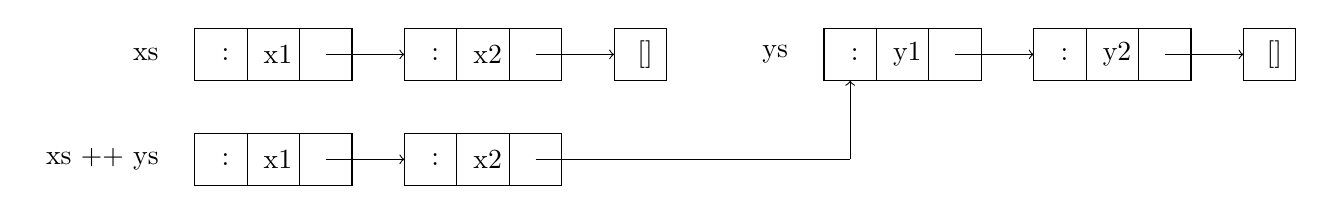
\begin{tikzpicture}[x=0.666cm, y=0.666cm]
                        \begin{scope}[shift={(0, 0)}]
                            \node[anchor=east] at (-0.5, -0.5) {~xs~};
                            \begin{scope}[shift={(0, 0)}]
                                \node at (0.5, -0.5) {~:~};
                                \node at (1.5, -0.5) {~x1~};
                                \draw
                                (0, 0) -- (3, 0) -- (3, -1) -- (0, -1) --cycle
                                (1, 0) -- (1, -1)
                                (2, 0) -- (2, -1)
                                (2.5, -0.5) edge[->] (4, -0.5);
                            \end{scope}
                            \begin{scope}[shift={(4, 0)}]
                                \node at (0.5, -0.5) {~:~};
                                \node at (1.5, -0.5) {~x2~};
                                \draw
                                (0, 0) -- (3, 0) -- (3, -1) -- (0, -1) --cycle
                                (1, 0) -- (1, -1)
                                (2, 0) -- (2, -1)
                                (2.5, -0.5) edge[->] (4, -0.5);
                            \end{scope}
                            \node at (8.5, -0.5) {~[]~};
                            \draw (8, 0) -- (9, 0) -- (9, -1) -- (8, -1) --cycle;
                        \end{scope}
                        \begin{scope}[shift={(12, 0)}]
                            \node[anchor=east] at (-0.5, -0.5) {~ys~};
                            \begin{scope}[shift={(0, 0)}]
                                \node at (0.5, -0.5) {~:~};
                                \node at (1.5, -0.5) {~y1~};
                                \draw
                                (0, 0) -- (3, 0) -- (3, -1) -- (0, -1) --cycle
                                (1, 0) -- (1, -1)
                                (2, 0) -- (2, -1)
                                (2.5, -0.5) edge[->] (4, -0.5);
                            \end{scope}
                            \begin{scope}[shift={(4, 0)}]
                                \node at (0.5, -0.5) {~:~};
                                \node at (1.5, -0.5) {~y2~};
                                \draw
                                (0, 0) -- (3, 0) -- (3, -1) -- (0, -1) --cycle
                                (1, 0) -- (1, -1)
                                (2, 0) -- (2, -1)
                                (2.5, -0.5) edge[->] (4, -0.5);
                            \end{scope}
                            \node at (8.5, -0.5) {~[]~};
                            \draw (8, 0) -- (9, 0) -- (9, -1) -- (8, -1) --cycle;
                        \end{scope}
                        \begin{scope}[shift={(0, -2)}]
                            \node[anchor=east] at (-0.5, -0.5) {~xs ++ ys~};
                            \begin{scope}[shift={(0, 0)}]
                                \node at (0.5, -0.5) {~:~};
                                \node at (1.5, -0.5) {~x1~};
                                \draw
                                (0, 0) -- (3, 0) -- (3, -1) -- (0, -1) --cycle
                                (1, 0) -- (1, -1)
                                (2, 0) -- (2, -1)
                                (2.5, -0.5) edge[->] (4, -0.5);
                            \end{scope}
                            \begin{scope}[shift={(4, 0)}]
                                \node at (0.5, -0.5) {~:~};
                                \node at (1.5, -0.5) {~x2~};
                                \draw
                                (0, 0) -- (3, 0) -- (3, -1) -- (0, -1) --cycle
                                (1, 0) -- (1, -1)
                                (2, 0) -- (2, -1);
                            \end{scope}
                            \draw
                            (6.5, -0.5) -- (12.5, -0.5)
                            (12.5, -0.5) edge[->] (12.5, 1);
                        \end{scope}
                    \end{tikzpicture}
                \end{center}
                Therefore, the complexity is linear, but only depends on ~xs~, and not ~ys~, hence we can say;
                \begin{center}
                    $T_~(++)~ \in O(n)$, where $n = ~length xs~$ in ~xs ++ ys~
                \end{center}
            \subsubsection*{Folding}
                The structure of lists is completed reduced by the ~foldr~ function;
                \begin{lstlisting}
                    foldr :: (a -> b -> b) -> b -> [a] -> b
                    foldr f k [] = k
                    foldr f k (x:xs) = f x (foldr f k xs)
                \end{lstlisting}
                This replaces ~(:)~ with ~f~, and ~[]~ with ~k~;
                \begin{center}
                    \begin{tikzpicture}
                        \begin{scope}[shift={(0, 0)}]
                            \node (o) at (0, 0) {~(:)~};
                            \node (ol) at (-1, -1) {~x1~};
                            \node (or) at (1, -1) {~(:)~};
                            \node (orl) at (0, -2) {~x2~};
                            \node (orr) at (2, -2) {~(:)~};
                            \node (orrl) at (1, -3) {~xn~};
                            \node (orrr) at (3, -3) {~[]~};
                            \draw
                            (o) -- (ol)
                            (o) -- (or)
                            (or) -- (orl)
                            (or) edge[thick, dotted] (orr)
                            (orr) -- (orrl)
                            (orr) -- (orrr);
                        \end{scope}
                        \node at (5, -1.5) {$\overset{~foldr f k~}{\leadsto}$};
                        \begin{scope}[shift={(8, 0)}]
                            \node (o) at (0, 0) {~f~};
                            \node (ol) at (-1, -1) {~x1~};
                            \node (or) at (1, -1) {~f~};
                            \node (orl) at (0, -2) {~x2~};
                            \node (orr) at (2, -2) {~f~};
                            \node (orrl) at (1, -3) {~xn~};
                            \node (orrr) at (3, -3) {~k~};
                            \draw
                            (o) -- (ol)
                            (o) -- (or)
                            (or) -- (orl)
                            (or) edge[thick, dotted] (orr)
                            (orr) -- (orrl)
                            (orr) -- (orrr);
                        \end{scope}
                    \end{tikzpicture}
                \end{center}
                Note that doing ~foldr (:) []~ is the same as ~id~, but with more work, and also ~xs ++ ys~ is equivalent to ~foldr (:) ys xs~.
                Similarly, we have ~foldl~;
                \begin{center}
                    \begin{minipage}[b]{0.55\textwidth}
                        \begin{lstlisting}
                            foldl :: (b -> a -> b) -> b -> [a] -> b
                            foldl f k [] = k
                            foldl f k (x:xs) = foldl f (f k s) xs
                        \end{lstlisting}
                    \end{minipage}
                    \hfill
                    \begin{minipage}[h]{0.4\textwidth}
                        \begin{center}
                            \begin{tikzpicture}[x=-1cm]
                                \node (o) at (0, 0) {~f~};
                                \node (ol) at (-1, -1) {~xn~};
                                \node (or) at (1, -1) {~f~};
                                \node (orl) at (0, -2) {~x2~};
                                \node (orr) at (2, -2) {~f~};
                                \node (orrl) at (1, -3) {~x1~};
                                \node (orrr) at (3, -3) {~k~};
                                \draw
                                (o) -- (ol)
                                (o) edge[thick, dotted] (or)
                                (or) -- (orl)
                                (or) -- (orr)
                                (orr) -- (orrl)
                                (orr) -- (orrr);
                            \end{tikzpicture}
                        \end{center}
                    \end{minipage}
                \end{center}
                Consider a binary operator $(\diamond)$;
                \begin{align*}
                    x \diamond (y \diamond z) & = (x \diamond y) \diamond z & \diamond-\text{associative} \\
                    \epsilon \diamond y & = y & \epsilon-\text{left-unit} \\
                    x \diamond \epsilon & = x & \epsilon-\text{right-unit}
                \end{align*}
                When folding with $\diamond$ and $\epsilon$, ~foldr~ and ~foldl~ coincide.
            \subsubsection*{List Concatenation}
                An application of this is list concatenation, consider ~concat~;
                \begin{lstlisting}
                    concat :: [[a]] -> [a]
                    concat [] = []
                    concat (xs:xss) = xs ++ concat xss
                \end{lstlisting}
                This can be written as a ~foldr~;
                \begin{lstlisting}
                    rconcat :: [[a]] -> [a]
                    rconcat = foldr (++) []
                \end{lstlisting}
                Since ~(++)~ is associate with a neutral element ~[]~, we can write a ~foldl~ version;
                \begin{lstlisting}
                    lconcat :: [[a]] -> [a]
                    lconcat = foldl (++) []
                \end{lstlisting}
                While ~lconcat = rconcat~, this only represents extensional (what values are produced) equality.
                They are not intensionally (how those values are produced) equal.
        \subsection*{18th October 2019}
            \subsubsection*{Concatenation and Associativity}
                The complexity of ~xs ++ ys~ is; $T_~(++)~(m, n) \in O(m)$, where $m = ~length xs~$, and $n = ~length ys~$ - note that it doesn't consider $n$ as expected.
                We want to consider the complexity of;
                $$\overbrace{~(~\underbrace{~(~\overbrace{~(~\underbrace{~(xs~_~1~~++ xs~_~2~~)~}_{n}~ ++ xs~_~3~~)~}^{2n}~ ++ ...)~}_{3n}~ ++ xs~_~m+1~~)~}^{mn}$$
                In lieu of having individual variables, we can approximate all the lists ~xs1~ to $~xs~_~m+1~$ as having the same length $n$.
                This means that if $m = ~length xss~$, then ~concat xss~ has complexity;
                \begin{center}
                    $n + 2n + 3n + \dots + mn = n(1 + 2 + 3 + \dots + m) \in O(nm^2)$
                \end{center}
                If we now look at the right associative version;
                \begin{center}
                    $~xs~_~1~~ ++ (xs~_~2~~ ++ (xs~_~3~~ ++ (... ++ (xs~_~m~~ ++ xs~_~{m+1}~~))))~$
                \end{center}
                Note that each of the ~++~ operations cost $n$, and we have $m$ of them, under the same assumption.
                Therefore, we have $O(mn)$.
                \medskip

                Note that adding to the right of a list is similar to doing the first version, which is left associative, and also more expensive.
                Preferably, we'd add to the left of the list, however this isn't always possible, as we'd also like to be able to add to the right of the list.
            \subsubsection*{Function Composition}
                We do not want to suffer the consequences of poor associativity.
                To solve this, we notice that function composition pays no associativity penalty.
                First note that function composition is as follows;
                \begin{center}
                    ~(f . g) x = f (g x)~
                \end{center}
                We can also show that function composition is both extensionally and intensionally equal, by unrolling the definition;
                \begin{center}
                    ~((f . g) . h) x = f (g (h x))~

                    vs

                    ~(f . (g . h)) x = f (g (h x))~
                \end{center}
                For our lists, we will replace with;
                \begin{center}
                    $~((xs~_~1~~ ++) . (xs~_~2~~ ++) . ... . (xs~_~m+1~~ ++)) []~$
                \end{center}
                Note that each of $~(xs~_~i~~ ++)~$ is a partially applied function that takes a list, and adds $~xs~_~i~$ to the start.
                This is equivalent to the right associative version we had before, which has a better time complexity.
            \subsubsection*{Difference List (DList)}
                The idea is to replace lists with functions that take in a list and give a list back.
                Previously, we'd consider $~xs~_~1~$ a list, but we now use $~(xs~_~1~~ ++)~$, which needs to be applied to the empty list.
                A value of type ~a~ in the list is now a function of type ~[a] -> [a]~.
                We can create a new datatype;
                \begin{lstlisting}
                    data DList a = DList ([a] -> [a])
                \end{lstlisting}
                We need ways of making lists from ~DList~s, and vice versa;
                \begin{lstlisting}
                    -- technically called the abstraction function
                    toList :: DList a -> [a]
                    toList (DList fxs) = fxs []

                    fromList :: [a] -> DList a
                    fromList xs = DList (xs ++)
                    -- or         DList (\ys -> xs ++ ys)
                \end{lstlisting}
                We also need a way of adding ~DList~s together (note the notes use $\diamond$, but I can't really get that with the listing environment, so I will use ~<>~);
                \begin{lstlisting}
                    (<>) :: DList a -> DList a -> DList a
                    DList fxs <> DList fys = DList (fxs . fys)
                    -- or                    DList (\zs -> fxs (fys zs))
                \end{lstlisting}
                Note that taking the head or tail of this list now requires constructing the entire list, which will take linear time.
            \subsubsection*{List Anatomy}
                \begin{center}
                    \begin{tikzpicture}[x=0.1cm]
                        \node[anchor=west] at (0, 0) {$~xs = [x~_~1~~, x~_~2~~, x~_~3~~, ..., x~_~n-1~~, x~_~n~~]~$};
                        \node (h) at (0, 1.25) {~head xs~};
                        \node (c) at (-10, -1) {\shortstack{(~x:~)\\~"cons"~}};
                        \node (l) at (79, -1.25) {~last xs~};
                        \node (s) at (89, 1) {\shortstack{(~++[y]~)\\~"snoc"~}};
                        \draw
                        (h) edge[bend left=20] (16, 0.5)
                        (c) edge[->, bend right=10] (10, -0.2)
                        (l) edge[bend left=20] (63, -0.5)
                        (s) edge[->, bend right=10] (69, 0.2);
                        \draw
                        (14, 0.5) edge[|-|] (18, 0.5)
                        (22, 0.5) edge[|-|, above] node{~tail xs~} (65, 0.5)
                        (65, -0.5) edge[|-|] (61, -0.5)
                        (57, -0.5) edge[|-|, below] node{~init xs~} (14, -0.5);
                    \end{tikzpicture}
                \end{center}
            \subsubsection*{List Interface}
                Rather than dealing with lists directly, we want to work with a specification instead.
                For this, we are creating a type class - an abstraction mechanism that has a class of objects, which have certain operations - and depending on what is given the operations can operate slightly differently.
                Note that ~List~ is the name of the type class, and ~list~ is the variable of abstraction.
                \begin{lstlisting}
                    class List list where
                    empty :: list a
                    cons :: a -> list a -> list a
                    snoc :: a -> list a -> list a
                    head :: list a -> a
                    tail :: list a -> list a
                    init :: list a -> list a
                    last :: list a -> a
                    length :: list a -> Int
                    (++) :: list a -> list a -> list a
                    null :: list a -> Bool
                    single :: list a -> Bool

                    toList :: list a -> [a]
                    fromList :: [a] -> list a
                \end{lstlisting}
                Note that ~toList~ and ~fromList~ must behave nicely when composed;
                \begin{center}
                    ~id = toList . fromList~
                \end{center}
                However, composing the functions in reverse does not necessarily yield the same result.
                Consider the case with our ~~DList - it would be perfectly valid to have ~(DList reverse)~; however, since the space of functions is much greater than the space of lists, we cannot reasonably convert ~revert~ into a list, and then hope to get ~reverse~ back out.
                \medskip

                However, we can say that if we had something representing a list, converting it to a list and then back to our implementation of a list, should yield something similar.
                \begin{center}
                    ~normalise = fromList . toList~
                \end{center}
            \subsubsection*{Exercises}
                \begin{enumerate}[1.]
                    \itemsep0em
                    \item Prove formally that $(n + 1)^2 \in \Theta(n^2)$ by exhibiting the necessary constants.
                        \medskip

                        We set $f(n) = (n + 1)^2$, and $g(n) = n^2$.
                        By our definition of $\Theta$, we need to satisfy both the following;
                        \begin{center}
                            $O(g(n)) = \{ f \bnfsep \violet{\exists \delta > 0.\ \exists n_0 > 0.\ \forall n > n_0.\ |f(n)| \leq \delta g(n)} \}$

                            $\Omega(g(n)) = \{f \bnfsep \teal{\exists \delta > 0.\ \forall n_0 > 0.\ \exists n > n_0.\ f(n) \geq \delta g(n)}\}$
                        \end{center}
                        The first case, we want to find $\delta$ such that;
                        \begin{align*}
                            (n + 1)^2 & \leq \delta n^2 & \Leftrightarrow \\
                            n^2 + 2n + 1 & \leq \delta n^2 & \Leftrightarrow \\
                            0 & \leq (\delta - 1) n^2 - 2n - 1 & \text{assuming } \delta - 1 = 3,\ \Rightarrow \\
                            0 & \leq (3n + 1)(n - 1)
                        \end{align*}
                        Hence we have $\delta = 4$.
                        The second case, $\Omega$, is trivial to prove with $\delta = 1$.
                    \item Give examples of expressions that are;
                        \begin{enumerate}[1.]
                            \itemsep0em
                            \item in head normal form, but not in normal form \hfill ~5:take 2 [1,2,3]~
                            \item in weak head normal form, but not in head normal form \hfill ~\ttbs x -> take 2 [1,2,3]~
                            \item in no normal form of any kind \hfill ~take 2 [1,2,3]~
                                \subitem it's not a constructor, and there isn't a $\lambda$-abstraction
                            \item in normal form, but not in weak head normal form \hfill not possible
                        \end{enumerate}
                    \item Using the definition of $f \in O(g(n))$ as a set, derive the definition of $f \in \omega(g(n))$ as a set.
                        \medskip

                        Recall that $f \in \omega(g(n)) \Leftrightarrow f \notin O(g(n))$, and the following definition;
                        \begin{center}
                            $O(g(n)) = \{ f \bnfsep \exists \delta > 0.\ \exists n_0 > 0.\ \forall n > n_0.\ |f(n)| \leq \delta g(n) \}$
                        \end{center}
                        Using equivalences for first-order logic;
                        \begin{align*}
                            & \neg \exists \delta > 0.\ \exists n_0 > 0.\ \forall n > n_0.\ |f(n)| \leq \delta g(n) \\
                            \equiv\ & \forall \delta > 0.\ \neg \exists n_0 > 0.\ \forall n > n_0.\ |f(n)| \leq \delta g(n) \\
                            \equiv\ & \forall \delta > 0.\ \forall n_0 > 0.\ \neg \forall n > n_0.\ |f(n)| \leq \delta g(n) \\
                            \equiv\ & \forall \delta > 0.\ \forall n_0 > 0.\ \exists n > n_0.\ \neg(|f(n)| \leq \delta g(n)) \\
                            \equiv\ & \forall \delta > 0.\ \forall n_0 > 0.\ \exists n > n_0.\ f(n) > \delta g(n)
                        \end{align*}
                        Hence we can write $\omega$ as the following;
                        \begin{center}
                            $\omega(g(n)) = \{ f \bnfsep \forall \delta > 0.\ \forall n_0 > 0.\ \exists n > n_0.\ f(n) > \delta g(n) \}$
                        \end{center}
                    \item
                        The composition rule gives the time complexity of two functions $f$ and $g$ when they are composed.
                        By using the definition of $e^T$, derive the accurate cost of $f\ (g\ x)$ using strict evaluation.
                        \begin{align*}
                            ((f \circ g)\ x)^T & = 1 + (f(g(x)))^T \\
                            & = 1 + f^T(g(x)) + (g(x))^T \\
                            & = 1 + f^T(g(x)) + g^Tx + x^T \\
                            & = 1 + f^T(g(x)) + g^Tx
                        \end{align*}
                    \item Justify whether each of the following is true or false;
                        \begin{enumerate}[1.]
                            \itemsep0em
                            \item $2n^2 + 3n \in \Theta(n^2)$ \hfill true
                            \item $2n^2 + 3n \in O(n^3)$ \hfill true
                            \item $n\log n \in O(n\sqrt{n})$ \hfill ($\log n$ grows slower than $\sqrt{n}$) true
                            \item $n + \sqrt{n} \in O(n\log n)$ \hfill false
                            \item $2^{\log n} \in O(n)$ \hfill (use laws of logarithms) true
                        \end{enumerate}
                \end{enumerate}
        \subsection*{22nd October 2020}
            \subsubsection*{Double-Ended Queues (Deque)}
                These are sometimes called symmetric lists.
                A normal list has the following complexities;
                \begin{center}
                    \begin{minipage}[t]{0.485\textwidth}
                        \begin{itemize}
                            \itemsep0em
                            \item ~cons x xs~ \hfill $O(1)$
                            \item ~head xs~ \hfill $O(1)$
                            \item ~tail xs~ \hfill $O(1)$
                        \end{itemize}
                    \end{minipage}
                    \hfill
                    \begin{minipage}[t]{0.485\textwidth}
                        \begin{itemize}
                            \itemsep0em
                            \item ~snoc x xs~ \hfill $O(n)$
                            \item ~last xs~ \hfill $O(n)$
                            \item ~init xs~ \hfill $O(n)$
                        \end{itemize}
                    \end{minipage}
                \end{center}
                We define a ~Deque~ as two lists, where the first list is in normal order, and the second list, containing the remainder of the whole list, is in reverse order (see the ~toList~ function)
                \begin{lstlisting}
                    data Deque a = Deque [a] [a]

                    toList :: Deque a -> [a]
                    toList (Deque xs ys) = xs ++ reverse ys
                \end{lstlisting}
                To add to the end of the list, we add to the front of the second list, hence we have constant time ~snoc~, as well as constant time ~cons~.
                \medskip

                To get desirable asymptotic complexities, there are two invariants that we require;
                \begin{itemize}
                    \itemsep0em
                    \item $~null xs~ \Rightarrow ~null ys~ \lor ~single ys~$
                    \item $~null ys~ \Rightarrow ~null xs~ \lor ~single xs~$
                \end{itemize}
                To make a ~Deque~ from a list, some symmetry is preferable.
                \begin{lstlisting}
                    fromList :: [a] -> Deque [a]
                    fromList xs = Deque us (reverse vs)
                      where
                        (us, vs) = splitAt (div n 2) xs
                        n = length xs
                \end{lstlisting}
                Some operations are easy to analyse and define;
                \begin{lstlisting}
                    snoc :: a -> Deque a -> Deque a
                    snoc y (Deque [] ys) = Deque ys [y]
                    snoc y (Deque xs ys) = Deque xs y:ys
                \end{lstlisting}
                This has $\Theta(1)$ complexity.
                It's important to note that we can do line 2 due to our invariant - if we know ~xs~ is empty, then ~ys~ must also be empty, or be a singleton list - and therefore it can be placed as the first list without a reversal.
                \begin{lstlisting}
                    last :: Deque a -> a
                    last (Deque xs []) = head xs -- or last xs
                    last (Deque xs y:ys) = y
                \end{lstlisting}
                This is also $O(1)$ complexity.
                Similarly, we know that ~xs~ is either empty (which would cause an error anyways), or it is singleton - thus the last item is the only item in the ~Deque~.
                \begin{lstlisting}
                    empty :: Deque a
                    empty = Deque [] []

                    tail :: Deque a -> Deque a
                    tail (Deque [] ys) = empty
                    tail (Deque [x] ys) = Deque (reverse vs) us
                      where
                        (us, vs) = splitAt (div n 2) ys
                        n = length ys
                    tail (Deque xs ys) = Deque (tail xs) ys
                \end{lstlisting}
                Here we define the empty ~Deque~, which is used in the first case (and doesn't cause an error).
                In the third case, we know that there is more than one element in ~xs~ (since it didn't match the second case), and therefore we simply take the tail (since we won't have an empty list, unlike the second case).
                In the second case, we discard the single ~x~.
                Symmetry is maintained by using the same split as ~fromList~.
                Note that ~ys~ is reversed, hence we can write $~ys = [y~_~n~~, y~_~n-1~~, ..., y~_~0~~]~$, and therefore $~(us, vs) = ([y~_~n~~, y~_~n-1~~, ..., y~_~j~~], [y~_~j-1~~, y~_~j-2~~, ..., y~_~0~~])~$, therefore ~vs~ needs to be reversed and put first.
                Both the first, and third cases are $O(1)$, but the worst case complexity is the second case, which has the reversal, and is $O(n)$.
            \subsubsection*{Amortised Analysis}
                In the worst case, the cost is $O(n)$, where $n = ~length ys~$.
                However, we rarely encounter this case.
                \medskip

                The idea of amortised analysis is that while it may have a high complexity in a single instance of the worst case, but it may not cost that amount in a sequence of operations.
                The cost of some functions is better expressed in terms of how it performs in a wider context.
                \medskip

                Consider repeated applications of ~tail~, in a chain (such that we apply ~tail~ to the result of the previous application) - each successive call to ~tail~ will cost less;
                \begin{center}
                    $~xs~_~0~ \overset{~tail~}{\leadsto} ~xs~_~1~ \overset{~tail~}{\leadsto} ~xs~_~2~ \overset{~tail~}{\leadsto} \dots \overset{~tail~}{\leadsto} ~xs~_~n~$
                \end{center}
                We can use amortised analysis to work out the true cost.
                \begin{center}
                    $~xs~_~0~ \overset{~op~_~0~}{\leadsto} ~xs~_~1~ \overset{~op~_~1~}{\leadsto} ~xs~_~2~ \overset{~op~_~2~}{\leadsto} \dots \overset{~op~_~n~}{\leadsto} ~xs~_~n+1~$
                \end{center}
                To perform amortised analysis, we need to define the following;
                \begin{itemize}
                    \itemsep0em
                    \item \textbf{cost} \hfill assign a real cost $C_{~op~_~i~}(~xs~_~i~)$ for each operation $~op~_~i~$ on data $~xs~_~i~$
                    \item \textbf{amortised cost} \hfill assign an amortised cost $A_{~op~_~i~}(~xs~_~i~)$ for each operation $~op~_~i~$ on data $~xs~_~i~$
                    \item \textbf{size} \hfill define $S(~xs~)$ that calculates the size of the data ~xs~
                \end{itemize}
                We use these to establish the following;
                $$\underbrace{\summation{i = 0}{n - 1} C_{~op~_~i~}(~xs~_~i~)}_\text{total actual cost} \leq \underbrace{\summation{i = 0}{n - 1} A_{~op~_~i~}(~xs~_~i~)}_\text{total amortised cost}$$
                For example, if we choose $A_{~op~_~i~}(~xs~_~i~) = 1$, then the total cost is $O(n)$.
                To prove this inequality (let it be equation (1)), we use the size function (physicist's approach);
                $$C_{~op~_~i~}(~xs~_~i~) \leq A_{~op~_~i~}(~xs~_~i~) + \overbrace{\underbrace{S(~xs~_~i~)}_\text{input size} - \underbrace{S(~xs~_~i+1~)}_\text{output size}}^\text{dif between data structure}$$
                We can sum over this as follows;
                $$\summation{i = 0}{n - 1} C_{~op~_~i~}(~xs~_~i~) \leq \summation{i = 0}{n - 1} A_{~op~_~i~}(~xs~_~i~) + S(~xs~_~0~) - S(~xs~_~n~)$$
                Let this be equation 2.
        \subsection*{25th October 2019}
            \subsubsection*{Size Function}
                One way of thinking about the size function is that it is similar to a bank; when a cheap operation is performed, we can put money in, and when an expensive operation is performed, we take money out.
                \medskip

                If we show equation 2, we have shown equation 1 - given that $S(~xs~_~0~) = 0$.
            \subsubsection*{Example on Deques}
                First, we can assign costs as follows;
                \begin{align*}
                    C_~cons~(~xs~) & = 1 \\
                    C_~snoc~(~xs~) & = 1 \\
                    C_~head~(~xs~) & = 1 \\
                    C_~last~(~xs~) & = 1 \\
                    C_~tail~(~Deque xs ys~) & = k & \text{where } k = ~length ys~
                \end{align*}
                Now, we can assign amortised costs.
                Regardless of the operation, we can say the charge is 2, hence we are overcharging by 1 for each of the constant time operations, in the hope that when we get to ~tail~, we have enough "saved up";
                \begin{center}
                    $A_~op~(~Deque xs ys~) = 2$
                \end{center}
                Finally, we can define the size function to be the difference in size of ~xs~ and ~ys~.
                The expensive operation of doing ~tail~ happens when one of the two lists is empty, and reversal has to be done.
                Once this "distance" increases to a certain amount, we have to charge the expensive operation.
                \begin{center}
                    $S(~Deque xs ys~) = | ~length xs~ - ~length ys~ |$
                \end{center}
                We can now attempt to prove equation 2.
                Given ~Deque xs' ys' = tail (Deque xs ys)~, we have the following sizes (in the worst case, where ~xs~ is a singleton list, and ~ys~ is of length $k$, and after the operation the difference is at most 1, since the list is (approximately) symmetric);
                \begin{align*}
                    S(~Deque xs ys~) & = k - 1 \\
                    S(~Deque xs' ys'~) & = 1
                \end{align*}
                Substituting gives the following;
                \begin{center}
                    $\underbrace{C_~tail~(~Deque xs ys~)}_{= k} \leq \underbrace{A_~tail~(~Deque xs ys~)}_{= 2} + \underbrace{S(~Deque xs ys~)}_{= k - 1} - \underbrace{S(~Deque xs' ys'~)}_{= 1}$

                    $\Leftrightarrow$

                    $k \leq 2 + (k - 1) - 1 = k$ (which is true)
                \end{center}
                Note that if we overcharged (had a number higher than 2), we'd still have a constant cost.
            \subsubsection*{Counting}
                \begin{center}
                    \begin{minipage}[t]{0.485\textwidth}
                        Once again, we encounter Peano numbers (see \textbf{CO142} from last year);
                        \begin{lstlisting}
                            data Peano = Zero | Succ Peano

                            inc :: Peano -> Peano
                            inc n = Succ n

                            -- notice this errors for Zero
                            dec :: Peano -> Peano
                            dec (Succ n) = n

                            add :: Peano -> Peano -> Peano
                            add Zero n = n
                            add (Succ m) n = Succ (add m n)
                        \end{lstlisting}
                    \end{minipage}
                    \hfill
                    \begin{minipage}[t]{0.485\textwidth}
                        This has a duality with lists;
                        \begin{lstlisting}
                            data [a] = [] | (:) a [a]

                            -- mirrors inc
                            cons :: a -> [a] -> [a]
                            cons x xs = x:xs

                            -- mirrors dec (notice the error case)
                            tail :: [a] -> [a]
                            tail (x:xs) = xs

                            -- mirrors add
                            (++) :: [a] -> [a] -> [a]
                            [] ++ ys = ys
                            (x:xs) ++ ys = x:(xs ++ ys)
                        \end{lstlisting}
                    \end{minipage}
                \end{center}
                Counting in binary is as follows (our representation has the least significant bit first);
                \begin{lstlisting}
                    type Binary = [Bit] -- [] is decimal 0
                    data Bit = 0 | 1

                    inc :: Binary -> Binary
                    inc [] = [1]
                    inc (0:bs) = 1:bs
                    inc (1:bs) = 0:inc bs
                \end{lstlisting}
                Notice that, in the worst case, ~inc~ has complexity $n$, where $n$ is the number of bits.
                Once again, doing amortised analysis, we define the following;
                \begin{align*}
                    C_~inc~(~bs~) & = t + 1 & \text{where } t = ~length (takeWhile (== 1) bs)~ \\
                    A_~inc~(~bs~) & = 2 & \text{overcharge for amortised cost} \\
                    S(~bs~) & = ~length (filter (== 1) bs)~
                \end{align*}
                Size function is some kind of measure of how much "money" we have in the "bank".
                We're "paying" when we have a lot of ~1~s, therefore for any ~1~ we put down, we have to pay for it later - hence we define the size function as the number of ~1~s in the bit string.
                Additionally, recall that having $S(~xs~_~0~) = 0$ allows us to show equation 1, by showing equation 2 (which can be done with the inequality, without the summation).
                \medskip

                Given ~bs' = inc bs~, we want to verify the following;
                $$\underbrace{C_~inc~(~bs~)}_{= t + 1} \leq \underbrace{A_~inc~(~bs~)}_{= 2} + \underbrace{S(~bs~)}_{= b} - \underbrace{S(~bs'~)}_{= b^\prime}$$
                Note that we can relate $b$ and $b^\prime$ as $b^\prime = b - t + 1$, since we flip all the leading ~1~s to ~0~s (hence the $- t$), and then flip a ~0~ to a ~1~ (hence the $+ 1$).
                By doing those substitutions, we can conclude the following;
                \begin{center}
                    $t + 1 \leq 2 + b - (b - t + 1) = t + 1$ (which is true)
                \end{center}
                Note that we want $A$ to be as tight of a bound as possible - while the inequality would still hold true if we set $A$ to be the number of bits, we'd end up with a poor estimate.
            \subsubsection*{Relation with Lists}
                Comparing binary numbers to Peano numbers, we are going up in powers of two, and therefore we can communicate larger numbers with less space.
                Relating this back to lists, searching for an item by traversing the entire list mirrors Peano numbers.
                \medskip

                Binary numbers are in the form;
                \begin{center}
                    $b_0 b_1 b_2 \dots b_n$ meaning $2^0b_0 + 2^1b_1 + 2^2b_2 + \dots 2^nb_n$
                \end{center}
                We will work with a list representation that has $1, 2, 4, \dots, 2^n$ elements.
                Therefore, for a list;
                \begin{center}
                    $~[t~_~0~~, t~_~1~~, ..., t~_~n~~]~$
                \end{center}
                We will store 1 element in the $~t~_~0~$ position, 2 elements in the $~t~_~1~$ position, and $2^n$ elements in the $~t~_~n~$ position.
                Depending on how many elements we want, we will either store or not store in these positions - consider having 6 elements; nothing will be stored in the $~t~_~0~$ position, but we will store 2 elements in $~t~_~1~$, and 4 elements in $~t~_~2~$.
                To do this, we will be using trees, which also gives us logarithmic access.
                \medskip

                Looking up in a list is expensive (takes $\Theta(k)$ instructions);
                \begin{lstlisting}
                    (!!) :: [a] -> Int -> a
                    (x:xs) !! 0 = x
                    (x:xs) !! k = xs !! (k - 1)
                \end{lstlisting}
                To improve upon this, we seek $O(\log n)$ instead.
            \subsubsection*{Trees}
                This can be done with trees (note that the ~Int~ in the ~Node~ constructor is the size of the tree);
                \begin{lstlisting}
                    data Tree a = Leaf a | Node Int (Tree a) (Tree a)
                \end{lstlisting}
                \begin{center}
                    \begin{tikzpicture}
                        \node (o) at (0, 0) {~4~};
                        \node (ol) at (-2, -1) {~2~};
                        \node (or) at (2, -1) {~2~};
                        \node (oll) at (-3, -2) {~'a'~};
                        \node (olr) at (-1, -2) {~'b'~};
                        \node (orl) at (1, -2) {~'c'~};
                        \node (orr) at (3, -2) {~'d'~};
                        \draw
                        (o) -- (ol) (o) -- (or)
                        (ol) -- (oll) (ol) -- (olr)
                        (or) -- (orl) (or) -- (orr);
                    \end{tikzpicture}
                \end{center}
                \begin{lstlisting}
                    size :: Tree a -> Int
                    size (Leaf x) = 1
                    size (Node n l r) = n
                \end{lstlisting}
                In lieu of taking the sum of the subtrees, we can simply maintain an invariant that has ~n~ be the size of the tree.
                This can be done with a \textbf{smart constructor};
                \begin{lstlisting}
                    node :: Tree a -> Tree a -> Tree a
                    node l r = Node (size l + size r) l r
                \end{lstlisting}
                We can imagine that this has an instance of the ~List~ class;
                \begin{lstlisting}
                    instance List Tree where
                      toList :: Tree a -> [a]
                      toList (Leaf x) = [x]
                      toList (Node n l r) = toList l ++ toList r -- we can do better here
                      ...
                      (!!) :: Tree a -> Int -> a
                      Leaf x !! 0 = x
                      Node n l r !! k
                        | k < m     = l !! k
                        | otherwise = r !! k - m
                        where
                          m = size l
                \end{lstlisting}
            \subsubsection*{Random Access Lists (RALists)}
                Lists can be represented using binary numbers as follows;
                \begin{lstlisting}
                    type RAList a = [Maybe (Tree a)]

                    instance List RAList where -- can't actually do this on type synonyms
                      toList :: RAList a -> [a]
                      toList = concat . map to
                        where
                          to :: Maybe (Tree a) -> [a]
                          to Nothing = []
                          to (Just t) = toList t -- note this is toList :: Tree a -> [a]
                      (!!) :: RAList a -> Int -> a
                      (Nothing : ts) !! k = ts !! k
                      (Just t : ts) !! k
                        | k < m     = t !! k -- (!!) for Tree (overloading)
                        | otherwise = ts !! k - m
                        where
                          m = size t
                \end{lstlisting}
                We have the following extensional equality;
                \begin{center}
                    ~toList txs !! k = txs !! k~ where ~tks :: RAList a~
                \end{center}
                However, the RHS performs better, as the LHS constructs the list, and then performs a walk down it.
                The complexity of ~(!!)~ (on ~RAList~) is $O(\log k)$.
                \medskip

                To implement ~cons~, we need to mirror ~inc~ on binary numbers;
                \begin{lstlisting}
                    cons :: a -> RAList a -> RAList a
                    cons x xs = consT (Leaf x) xs
                      where
                        consT :: Tree a -> RAList a -> RAList a
                        consT t [] = [Just t]
                        consT t (Nothing:ts) = (Just t):ts
                        consT t ((Just t'):ts) = Nothing:consT (node t t') ts
                \end{lstlisting}
        \subsection*{29th October 2019}
            \subsubsection*{Divide and Conquer, Merge Sort}
                This strategy has the following three parts;
                \begin{enumerate}[1.]
                    \itemsep0em
                    \item divide a problem into subproblems
                    \item apply the strategy to subproblems to make subsolutions
                    \item combine subsolutions to make a solution
                \end{enumerate}
                A classic example is merge sort;
                \begin{lstlisting}
                    msort :: [Int] -> [Int]
                    msort [] = []
                    msort [x] = [x]
                    msort xs = merge (msort us) (msort vs)
                      where
                        (us, vs) = splitAt (div n 2) xs
                        n = length xs

                    merge :: [Int] -> [Int] -> [Int]
                    merge [] ys = ys
                    merge xs [] = xs
                    merge (x:xs) (y:ys)
                      | x <= y    = x:merge xs (y:ys)
                      | otherwise = y:merge (x:xs) ys
                \end{lstlisting}
                We can perform the following recurrence relation to obtain the complexity;
                \begin{align*}
                    T_~msort~(0) & = 1 \\
                    T_~msort~(1) & = 1 \\
                    T_~msort~(n) & = \underbrace{T_~length~(n)}_{O(n)} + \underbrace{T_~splitAt~\left(\frac{n}{2}\right)}_{O(n)} + \underbrace{T_~merge~\left(\frac{n}{2}\right)}_{O(n)} + 2 \cdot T_~msort~\left(\frac{n}{2}\right)
                \end{align*}
                For this, we can draw a recursion tree to represent the structure (note the initial $c \cdot n$ represents the three $O(n)$ costs combined, and so on);
                \begin{center}
                    \begin{tikzpicture}[x=2cm]
                        \node (o) at (0, 0) {$c \cdot n$};
                        \node (ol) at (-1, -1) {$c \cdot \frac{n}{2}$};
                        \node (or) at (1, -1) {$c \cdot \frac{n}{2}$};
                        \node (oll) at (-1.5, -2) {$c \cdot \frac{n}{4}$};
                        \node (olr) at (-0.5, -2) {$c \cdot \frac{n}{4}$};
                        \node (orl) at (0.5, -2) {$c \cdot \frac{n}{4}$};
                        \node (orr) at (1.5, -2) {$c \cdot \frac{n}{4}$};
                        \node (olld) at (-1.5, -3) {$c$};
                        \node (olrd) at (-0.5, -3) {$c$};
                        \node (orld) at (0.5, -3) {$c$};
                        \node (orrd) at (1.5, -3) {$c$};
                        \node at (-1, -3) {$\cdots$};
                        \node at (0, -3) {$\cdots$};
                        \node at (1, -3) {$\cdots$};
                        \draw
                        (o) -- (ol) (o) -- (or)
                        (ol) -- (oll) (ol) -- (olr)
                        (or) -- (orl) (or) -- (orr)
                        (oll) edge[thick, dotted] (olld)
                        (olr) edge[thick, dotted] (olrd)
                        (orl) edge[thick, dotted] (orld)
                        (orr) edge[thick, dotted] (orrd);
                        \draw
                        (-1.75, -3.5) edge[|-|, below] node{$n$} (1.75, -3.5)
                        (2, 0) edge[|-, right] node{$\log_2 n$} (2, -2)
                        (2, -2) edge[dashed, -|] (2, -3);
                    \end{tikzpicture}
                \end{center}
                Therefore, we can conclude the following; \hfill $T_~msort~(n) \in \Theta(n\log n)$
            \subsubsection*{Quicksort}
                For this implementation, we will use the head of the list as the pivot - using an arbitrary element is better.
                \begin{lstlisting}
                    qsort :: [Int] -> [Int]
                    qsort [] = []
                    qsort [x] = [x]
                    qsort (x:xs) = qsort us ++ [x] ++ qsort vs
                      where
                        (us, vs) = partition (< x) xs

                    partition :: (a -> Bool) -> [a] -> ([a], [a])
                    partition p xs = (filter p xs, filter (not . p) xs)
                \end{lstlisting}
                In the best case, the cost is the same as ~msort~, since we are splitting the list in the middle.
                However, in the worst case we have the following;
                \begin{align*}
                    T_~qsort~(n) & = \underbrace{T_~partition~(n)}_{O(n)} + \underbrace{T_~(++)~(n - 1)}_{O(n)} + T_~qsort~(1) + T_~qsort~(n - 1) \\
                    & = c \cdot n + T_~qsort~(n - 1) \\
                    & = \underbrace{c \cdot n + c \cdot n + \dots + c \cdot n}_n + 1 \\
                    & = c \cdot n^2 + 1
                \end{align*}
                Hence $T_~qsort~ \in O(n^2)$.
            \subsubsection*{Binary Search Trees / AVL Trees}
                \begin{center}
                    \begin{minipage}[h]{0.6\textwidth}
                        We start with a tree which mirrors ~qsort~;
                        \begin{lstlisting}
                            data QTree a = QNil | Node (QTree a) a (QTree a)
                        \end{lstlisting}
                        The idea is that, for the diagram on the right, elements in $l$ are less than $x$ and elements in $r$ are greater than $x$;
                    \end{minipage}
                    \hfill
                    \begin{minipage}[h]{0.3\textwidth}
                        \begin{center}
                            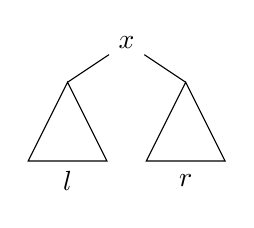
\begin{tikzpicture}[x=0.5cm, y=0.5cm]
                                \node (x) at (0, 0) {$x$};
                                \node at (-1.5, -3.5) {$l$};
                                \node at (1.5, -3.5) {$r$};
                                \draw (x) -- (-1.5, -1) (x) -- (1.5, -1);
                                \draw (-1.5, -1) -- (-0.5, -3) -- (-2.5, -3) -- cycle;
                                \draw (1.5, -1) -- (2.5, -3) -- (0.5, -3) -- cycle;
                            \end{tikzpicture}
                        \end{center}
                    \end{minipage}
                \end{center}
                \begin{lstlisting}
                    fromList :: [Int] -> QTree Int
                    fromList [] = QNil
                    fromList (x:xs) = QNode (fromList us) x (fromList vs)
                      where
                        (us, vs) = partition (< x) xs
                \end{lstlisting}
                Notice that this essentially encapsulates the call structure of ~qsort~ in memory.
                Flattening this tree will give us a sorted list, equivalent to ~qsort~.
                The ~fromList~ function has the same complexity as ~qsort~, which is $O(n \log n)$ in the best case, and $O(n^2)$ in the worst case.
                \medskip

                The goal is to change the data structure so that it takes $O(n \log n)$ on average.
                To achieve this performance, we want to keep the tree balanced - hence we want to store the height of the tree (in lieu of traversing it, since we will use this operation frequently).
                A binary search tree has this representation (with the ~Int~ representing height, and a smart constructor ~bnode~ to maintain this property);
                \begin{lstlisting}
                    data BTree a = BNil | BNode Int (BTree a) a (BTree a)

                    height :: BTree a -> Int
                    height BNil = 0
                    height (BNode h l x r) = h

                    bnode :: BTree a -> a -> BTree a -> BTree a
                    bnode l x r = BNode h l x r
                      where
                        h = 1 + max (height l) (height r)
                \end{lstlisting}
                The algorithm will consist of repeated inserts into the tree - the ~fromList~ function will take a list of elements and ~foldr~ over it.
                The ~insert~ function must maintain the balance of the tree.
                \begin{lstlisting}
                    fromList :: [Int] -> BTree Int
                    fromList xs = foldr insert BNil

                    insert :: Int -> BTree Int -> BTree Int
                    insert x BNil = bnode BNil x BNil
                    insert x (BNode h l y r)
                      | x < y  = balance (insert x l) y r
                      | x == y = BNode h l y r -- discarding if equal
                      | x > y  = balance x y (insert x r)
                \end{lstlisting}
                Note that ~balance~ is another smart constructor.
        \subsection*{1st November 2019}
            \subsubsection*{BTrees (Continued)}
                The intuition is that the tree given to ~insert~ is roughly balanced, such that the difference in heights of the left and right subtrees are at most 1.
                We define a tree to be \textbf{biased} if its subtrees differ in height;
                \begin{lstlisting}
                    bias :: BTree a -> Int
                    bias BNil = 0
                    bias (BNode h l x r) = height l - height r
                \end{lstlisting}
                Therefore, we are \violet{off by at most 2} after performing the insertion.
                The ~balance~ smart construction ensures the trees are balanced when they are originally \violet{off by at most 2};
                \begin{lstlisting}
                    balance :: BTree Int -> Int -> BTree Int -> BTree Int
                \end{lstlisting}
                Given ~balance l x r~, we have the following cases;
                \begin{enumerate}[1.]
                    \itemsep0em
                    \item trees differ by at most 1;
                        \begin{enumerate}[(a)]
                            \itemsep0em
                            \item the tree is balanced
                                \begin{center}
                                    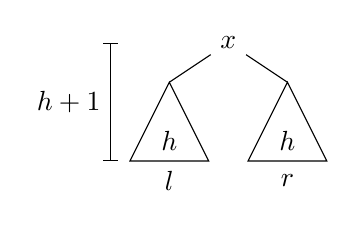
\begin{tikzpicture}[x=0.5cm, y=0.5cm]
                                        \node (x) at (0, 0) {$x$};
                                        \avltri{-1.5, -1}{$l$}{$h$}{2}
                                        \avltri{1.5, -1}{$r$}{$h$}{2}
                                        \draw (x) -- (-1.5, -1) (x) -- (1.5, -1);
                                        \draw(-3, -3) edge[|-|, left] node{$h + 1$} (-3, 0);
                                    \end{tikzpicture}
                                \end{center}
                            \item the tree is off by 1 (showing only left tree being larger, without loss of generality)
                                \begin{center}
                                    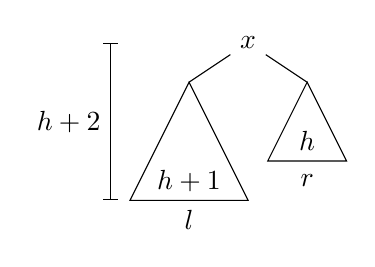
\begin{tikzpicture}[x=0.5cm, y=0.5cm]
                                        \node (x) at (0, 0) {$x$};
                                        \avltri{-1.5, -1}{$l$}{$h + 1$}{3}
                                        \avltri{1.5, -1}{$r$}{$h$}{2}
                                        \draw (x) -- (-1.5, -1) (x) -- (1.5, -1);
                                        \draw (-3.5, -4) edge[|-|, left] node{$h + 2$} (-3.5, 0);
                                    \end{tikzpicture}
                                \end{center}
                        \end{enumerate}
                        Regardless, this is fine, hence ~balance l x r = bnode l x r~
                    \item the trees are biased by 2;
                        \begin{enumerate}[(a)]
                            \itemsep0em
                            \item assume that $~height l~ > ~height r~$, and also $~height height ll~ \geq ~height rl~$ (where ~rl~ is the right subtree of the left subtree)
                                \begin{center}
                                    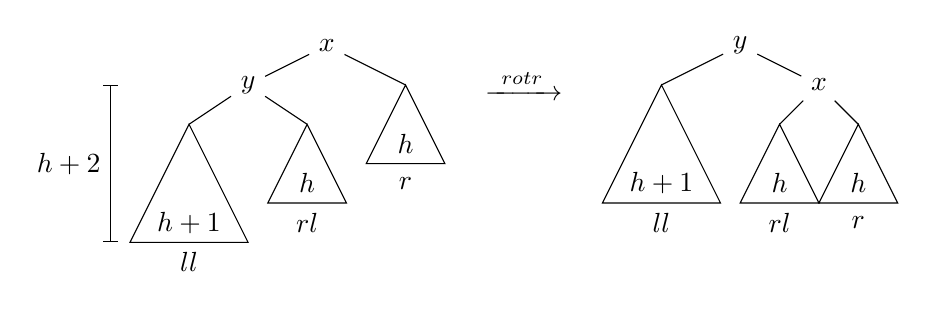
\begin{tikzpicture}[x=0.5cm, y=0.5cm]
                                        \node at (5, -1) {$\xrightarrow{~rotr~}$};
                                        \begin{scope}[shift={(0, 0)}]
                                            \node (x) at (0, 0) {$x$};
                                            \node (y) at (-2, -1) {$y$};
                                            \coordinate (ll) at (-3.5, -2);
                                            \coordinate (rl) at (-0.5, -2);
                                            \coordinate (r) at (2, -1);
                                            \avltri{r}{$r$}{$h$}{2}
                                            \avltri{ll}{$ll$}{$h + 1$}{3}
                                            \avltri{rl}{$rl$}{$h$}{2}
                                            \draw
                                            (x) -- (y) (x) -- (2, -1)
                                            (y) -- (ll) (y) -- (rl);
                                            \draw (-5.5, -5) edge[|-|, left] node{$h + 2$} (-5.5, -1);
                                        \end{scope}
                                        \begin{scope}[shift={(10.5, 0)}]
                                            \node (y) at (0, 0) {$y$};
                                            \node (x) at (2, -1) {$x$};
                                            \coordinate (ll) at (-2, -1);
                                            \coordinate (rl) at (1, -2);
                                            \coordinate (r) at (3, -2);
                                            \avltri{ll}{$ll$}{$h + 1$}{3}
                                            \avltri{rl}{$rl$}{$h$}{2}
                                            \avltri{r}{$r$}{$h$}{2}
                                            \draw
                                            (y) -- (ll) (y) -- (x)
                                            (x) -- (rl) (x) -- (r);
                                        \end{scope}
                                    \end{tikzpicture}
                                \end{center}
                                \begin{lstlisting}
                                    balance l x r = rotr (node l x r)

                                    rotr :: BTree a -> BTree a
                                    rotr (BNode _ (BNode _ ll y rl) x r)
                                      = bnode ll y (bnode rl x r)
                                \end{lstlisting}
                            \item assume that $~height l~ > ~height r~$, and also $~height height ll~ < ~height rl~$;
                                \begin{center}
                                    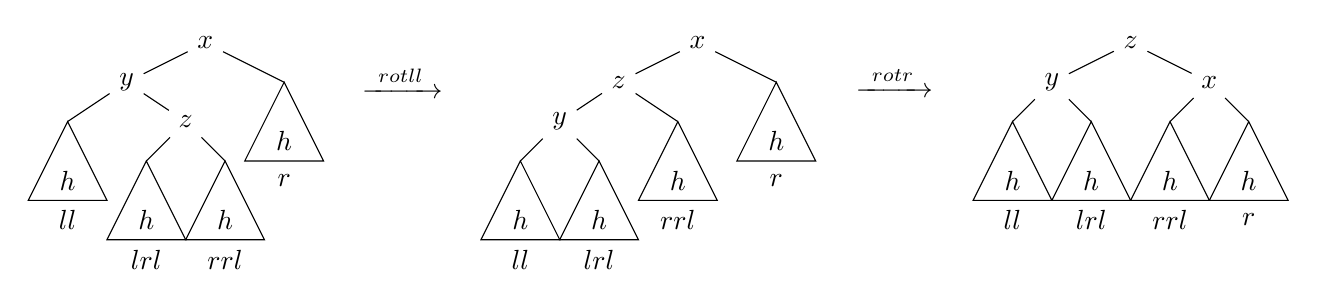
\begin{tikzpicture}[x=0.5cm, y=0.5cm]
                                        \node at (5, -1) {$\xrightarrow{~rotl l~}$};
                                        \node at (17.5, -1) {$\xrightarrow{~rotr~}$};
                                        \begin{scope}[shift={(0, 0)}]
                                            \node (x) at (0, 0) {$x$};
                                            \node (y) at (-2, -1) {$y$};
                                            \node (z) at (-0.5, -2) {$z$};
                                            \coordinate (ll) at (-3.5, -2);
                                            \coordinate (lrl) at (-1.5, -3);
                                            \coordinate (rrl) at (0.5, -3);
                                            \coordinate (r) at (2, -1);
                                            \avltri{r}{$r$}{$h$}{2}
                                            \avltri{ll}{$ll$}{$h$}{2}
                                            \avltri{lrl}{$lrl$}{$h$}{2}
                                            \avltri{rrl}{$rrl$}{$h$}{2}
                                            \draw
                                            (x) -- (y) (x) -- (r)
                                            (y) -- (ll) (y) -- (z)
                                            (z) -- (lrl) (z) -- (rrl);
                                        \end{scope}
                                        \begin{scope}[shift={(12.5, 0)}]
                                            \node (x) at (0, 0) {$x$};
                                            \node (z) at (-2, -1) {$z$};
                                            \node (y) at (-3.5, -2) {$y$};
                                            \coordinate (ll) at (-4.5, -3);
                                            \coordinate (lrl) at (-2.5, -3);
                                            \coordinate (rrl) at (-0.5, -2);
                                            \coordinate (r) at (2, -1);
                                            \avltri{r}{$r$}{$h$}{2}
                                            \avltri{ll}{$ll$}{$h$}{2}
                                            \avltri{lrl}{$lrl$}{$h$}{2}
                                            \avltri{rrl}{$rrl$}{$h$}{2}
                                            \draw
                                            (x) -- (z) (x) -- (r)
                                            (z) -- (y) (z) -- (rrl)
                                            (y) -- (ll) (y) -- (lrl);
                                        \end{scope}
                                        \begin{scope}[shift={(23.5, 0)}]
                                            \node (z) at (0, 0) {$z$};
                                            \node (y) at (-2, -1) {$y$};
                                            \node (x) at (2, -1) {$x$};
                                            \coordinate (ll) at (-3, -2);
                                            \coordinate (lrl) at (-1, -2);
                                            \coordinate (rrl) at (1, -2);
                                            \coordinate (r) at (3, -2);
                                            \avltri{r}{$r$}{$h$}{2}
                                            \avltri{ll}{$ll$}{$h$}{2}
                                            \avltri{lrl}{$lrl$}{$h$}{2}
                                            \avltri{rrl}{$rrl$}{$h$}{2}
                                            \draw
                                            (z) -- (y) (z) -- (x)
                                            (y) -- (ll) (y) -- (lrl)
                                            (x) -- (rrl) (x) -- (r);
                                        \end{scope}
                                    \end{tikzpicture}
                                \end{center}
                                \begin{lstlisting}
                                    balance l x r = rotr (node (rotl l) x r)

                                    rotl :: BTree a -> BTree a
                                    rotl (BNode _ ll y (BNode _ lrl z rrl))
                                      = bnode (bnode ll y lrl) z rrl
                                \end{lstlisting}
                        \end{enumerate}
                \end{enumerate}
                Putting all of this together;
                \begin{lstlisting}
                    balance :: BTree a -> a -> BTree a -> BTree a
                    balance l x r
                      | abs b <= 1 = bnode l x r                       -- (case 1a, 1b)
                      | b == 2     =
                          if 0 <= bias l then rotr (node l x r)        -- (case 2a)
                                         else rotr (node (rotl l) x r) -- (case 2b)
                      | b == -2    =
                          if bias r <= 0 then rotl (node l x r)        -- (symmetry of 2a)
                                         else rotl (node l x (rotr r)) -- (symmetry of 2b)
                \end{lstlisting}
                Since ~balance~, ~rotr~, and ~rotl~ have no recursion, and are straight pattern matches, the process of balancing a tree is constant time.
                \medskip

                However, we have recursion in ~insert~.
                Since we have balanced the tree, we can therefore say that the size of the left and right subtrees are roughly equal, hence the height of the tree is approximately $\log_2 n$; and since we are doing a constant time operation at each level;
                \begin{center}
                    $T_~insert~(n) \in O(\log n)$
                \end{center}
                Similarly, since it is a balanced tree, looking up values is also $O(\log n)$.
                \medskip

                By our definition of ~fromList~, we are folding over a list of size $n$, and performing a $\log n$ operation for each, hence we have $O(n \log n)$.
            \subsubsection*{Sorting with BTrees}
                Since the tree is ordered, we a natural sorting algorithm;
                \begin{center}
                    ~sort = toList . fromList~
                \end{center}
                Since we already know ~fromList~ is $O(n \log n)$, ~toList~ is the limiting factor - if we can get it to $O(n \log n)$ or better, the overall cost of the sort is $O(n \log n)$.
                \begin{lstlisting}
                    toList :: BTree a -> [a]
                    toList BNil = []
                    toList (Node _ l x r) = toList l ++ [x] ++ toList r
                \end{lstlisting}
                Assuming we made ~toList~ use $O(n)$ time (the implementation above takes $O(n^2)$, but we could've used a ~DList~), we cannot get a better ~fromList~, since it would lower the overall cost of ~sort~ to $O(n)$, which isn't possible due to a lower bound on sorting algorithms.
                \medskip

                Recall that ~DList~ uses function composition, which gives preferable associativity.
                Therefore, we want the following;
                \begin{center}
                    ~toList l ++ [x] ++ toList r~

                    $\downarrow$

                    ~(toList' l . (x:) . toList' r) []~
                \end{center}
                Note that the function ~toList'~ takes a ~BTree a~, and gives a \textbf{function} that takes a ~[a]~ and gives back ~[a]~;
                \begin{lstlisting}
                    toList' :: BTree a -> ([a] -> [a])
                    toList' BNil xs = xs
                    toList' (BNode _ l x r) xs = (toList' l . (x:) . toList' r) xs
                \end{lstlisting}
                Therefore, we can write the following;
                \begin{lstlisting}
                    toList t = toList' t []
                \end{lstlisting}
                Hence our ~toList~ is $O(n)$.
            \subsubsection*{Dynamic Programming}
                The idea behind dynamic programming is that we start with a recursive function, and repeated calls do not get executed again.
                We are trading space for speed.
                An example is calculating Fibonacci numbers (note that ~Int~ is bounded by the CPU, and ~Integer~ is larger and bounded by RAM);
                \begin{lstlisting}
                    fib :: Int -> Integer
                    fib 0 = 0
                    fib 1 = 1
                    fib n = fib (n - 1) + fib (n - 2)
                \end{lstlisting}
                \begin{center}
                    \begin{tikzpicture}[x=2cm]
                        \node (o) at (0, 0) {~fib 10~};
                        \node (ol) at (-2, -1) {~fib 8~};
                        \node (or) at (2, -1) {~fib 9~};
                        \node (oll) at (-3, -2) {~fib 6~};
                        \node (olr) at (-1, -2) {~fib 7~};
                        \node[red] (orl) at (1, -2) {~fib 7~};
                        \node[red] (orr) at (3, -2) {~fib 8~};
                        \node (olld) at (-3, -3) {$\vdots$};
                        \node (olrd) at (-1, -3) {$\vdots$};
                        \node (orld) at (1, -3) {$\vdots$};
                        \node (orrd) at (3, -3) {$\vdots$};
                        \draw
                        (o) -- (ol) (o) -- (or)
                        (ol) -- (oll) (ol) -- (olr)
                        (or) -- (orl) (or) -- (orr)
                        (oll) -- (olld)
                        (olr) -- (olrd)
                        (orl) -- (orld)
                        (orr) -- (orrd);
                    \end{tikzpicture}
                \end{center}
                However, notice that some values are recomputed, which wastes time.
                Ideally, we'd want to store the values we compute in a table, giving us constant time lookup.
\end{document}